\subsection{Modelo Conceptual}

\begin{figure}
  \begin{center}
	%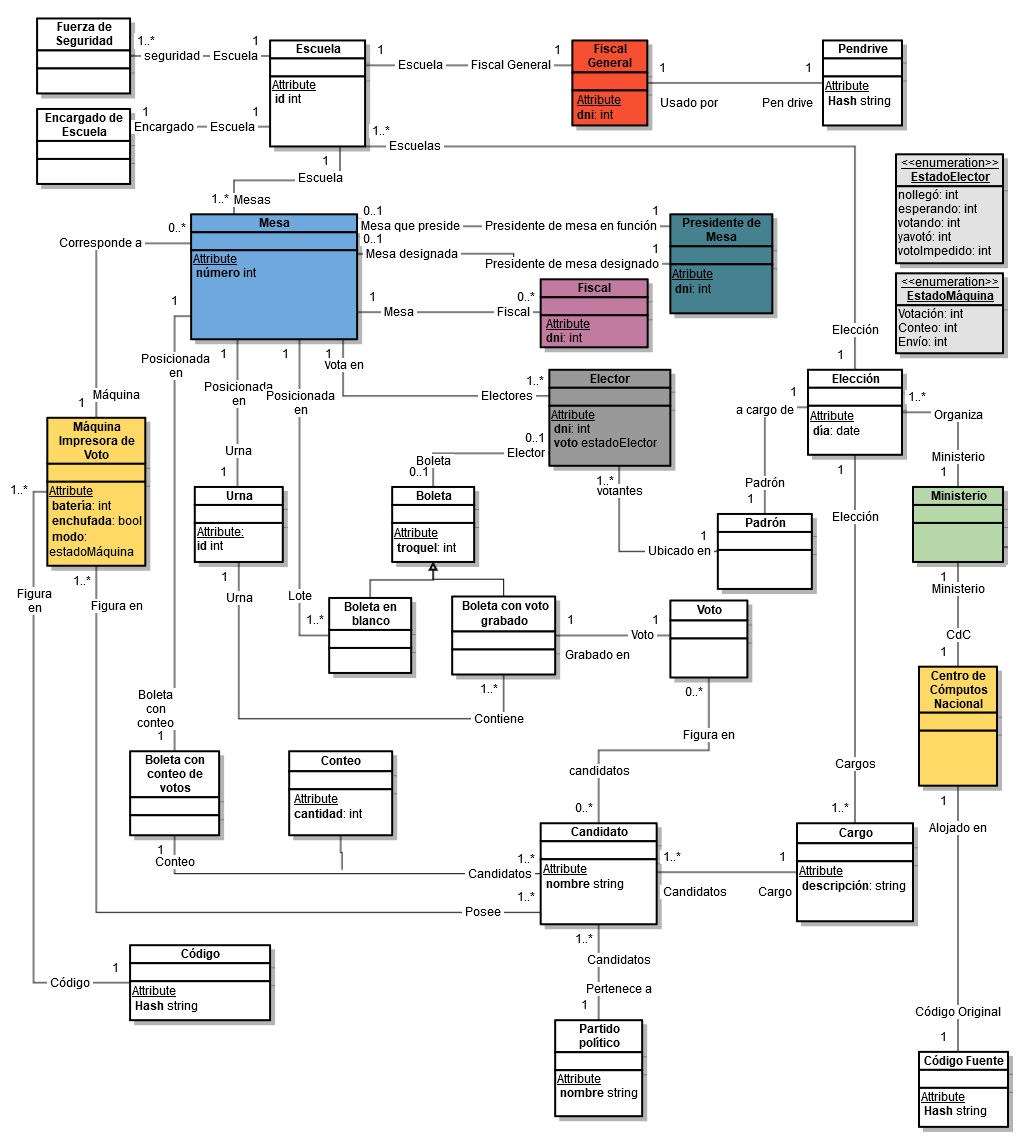
\includegraphics[scale=0.64]{imagenes/clases.png}
  \end{center}
\end{figure}

\newpage
\subsubsection{OCL}


\subsubsection*{Mesa}

\textit{context Mesa
inv}
\begin{enumerate}

\item Los n\'umeros de las mesas son únicos.

$Mesa.AllInstances \rightarrow forAll(m_1, m_2 | m_1<>m_2$ implies $m_1.numero <> m_2.numero))$

\item  No hay dos mesas con el mismo fiscal.\textcolor{red}{Preguntar si esto esta bien...}

$Mesa.AllInstances \rightarrow forAll(m_1, m_2 | m_1<>m_2$ implies $m_1.Fiscal.dni <> m_2.Fiscal.dni))$

\item No hay dos mesas con electores en común.

$Mesa.AllInstances \rightarrow \\
 forAll(m_1, m_2 | m_1<>m_2$ implies $m_1.Electores \rightarrow \\
 	forAll(e_1 | m_2.Electores \rightarrow Select(e_2 | e_2 <> e_1) \rightarrow Size() == 0))$

\item No hay dos mesas con el mismo presidente de mesa.

$Mesa.AllInstances \rightarrow \\
forAll(m_1, m_2 | m_1<>m_2$ implies $ \\ m_1.PresidenteDeMesaDesignado.dni <> m_2.PresidenteDeMesaDesignado.dni))$

\item Los presidentes de mesa votan en la misma mesa que son presidentes.

$self.Electores \rightarrow Select(e | self.PresidenteDeMesaDesignado.dni == e.dni) \rightarrow Size() ==1$


\item La cantidad de Boletas Sin voto grabado y con voto grabado de la mesa debe ser mayor o igual a la cantidad de electores de dicha mesa.

$self.Lote \rightarrow Size() + self.Urna.Contiene \rightarrow Size () \geq self.Electores \rightarrow Size()$

\item La cantidad de Boletas Con voto grabado de la mesa debe ser menor o igual a la cantidad de electores de dicha mesa.

$self.Urna.Contiene  \rightarrow  Size() \leq self.Electores \rightarrow Size()$

\item Si la máquina está en modo votación es porque s\'olo un elector, o ninguno, está votando.

$self.Maquina.modo == votacion$ implies $ \\
self.Electores \rightarrow select(e | e.voto == votando) \rightarrow Size() \leq 1$

\item Si la máquina está en modo conteo es porque no hay ningún elector de la mesa votando o esperando para votar.\textcolor{red}{Ver OR}

$self.Maquina.modo == votacion$ implies $ \\
self.Electores \rightarrow \\
select(e | e.voto == votando OR e.voto == esperando) \rightarrow Size() = 0$

\item La máquina de la mesa puede estar en modo votación o conteo pero no en envio.\textcolor{red}{Ver !}

$!self.Maquina.modo == envio$

\item No puede haber un fiscal y un presidente de mesa con el mismo dni.

$self.Fiscales \rightarrow \\
select(f | f.dni == self.PresidenteDeMesaEnFuncion.dni OR \\
f.dni == self.PresidenteDeMesaDesignado.dni) \rightarrow \\
Size() == 0 $


\end{enumerate}

\subsubsection*{Boleta}
\begin{enumerate}

\item Los id de las boletas son únicos.

$Boleta.AllInstances() \rightarrow select(b_1, b_2 | b_1 <> b_2 $ implies $ b_1.troquel <> b_2.troquel)$

\item La boleta con voto grabado tiene elector.


\item Si un elector tiene una boleta en blanco, entonces esta boleta está en la mesa que el elector vota.\textcolor{red}{Ver AND}

$self.IsKindOf(BoletaEnBlanco)? AND self.Elector \rightarrow Size() == 1 $ implies $\\
self.PosicionadaEn.numero == self.Elector.VotaEn.numero$

\item Si un elector tiene una boleta con voto grabado, entonces esta boleta está en la urna que el elector vot\'o.

$self.IsKindOf(BoletaConVotoGrabado)? $ implies $\\
self.Urna.PosicionadaEn.numero == self.Elector.VotaEn.numero$

\end{enumerate}


\subsubsection*{Conteo}

\begin{enumerate}

\item La boleta con conteo realmente tiene la información de las boletas de la urna (o sea la suma de los candidatos que hayan votado).
$self.Cantidad == \\
self.BoletaConConteodeVotos.mesa.boletaConVotoGrabado \rightarrow \\
select(b | b.voto.candidato  \rightarrow exist(c | c==self.candidato)) \rightarrow size() $
\end{enumerate}

\subsubsection*{Voto}
\begin{enumerate}
\item No tiene dos candidatos con el mismo cargo.

\item No tiene dos candidatos con el mismo nombre.
\end{enumerate}

\subsubsection*{Urna}
\begin{enumerate}
\item Las boletas con voto grabado de la urna son sólo de votantes de la mesa que figura la urna.
\item En una misma urna no hay dos boletas con el mismo elector.    
\item Los id de las urnas son únicos.
\end{enumerate}

\subsubsection*{Escuela}
\begin{enumerate}
\item Los id de las mesas son únicos.
\item No puede haber un fiscal general y un fiscal con el mismo dni.
\item No puede haber un fiscal general y un presidente de mesa con el mismo dni.
\end{enumerate}

\subsubsection*{M\'aquina Impresora de Voto}
\begin{enumerate}
\item Los candidatos de todas las máquinas son los mismos.

\end{enumerate}

\subsubsection*{Elector}
\begin{enumerate}
\item Los dni de los electores son únicos.
\item El elector puede no tener ninguna boleta, tener una vacía o tener una con voto.
\item No puede haber un elector y una persona que no figura en el padrón con el mismo dni.
\item Si el elector no llegó, está esperando o no lo dejaron votar no tiene boleta.
\item Si el elector está votando tiene una boleta en blanco.
\item Si el elector ya votó tiene una boleta con voto grabado.
\end{enumerate}

\subsubsection*{Partido Pol\'itico}
\begin{enumerate}
\item No hay dos partidos políticos con ningún candidato en común.
\end{enumerate}

\subsubsection*{Centro de C\'omputos}
\begin{enumerate}
\item Hay uno solo.
\end{enumerate}

\subsubsection*{C\'odigo}
\begin{enumerate}
\item El hash del código es el mismo del hash del código fuente.   
\item El hash del código es el mismo del hash de todos los pendrives de los fiscales.   
\end{enumerate}  

\subsubsection*{Ministerio}
\begin{enumerate}
\item Hay un solo ministerio.
\end{enumerate}

\subsubsection*{Equipo T\'ecnico}
\begin{enumerate}
\item Hay uno sólo.
\end{enumerate}

\subsubsection*{Presidente de Mesa}
\begin{enumerate}
\item Si el presidente de mesa del ministerio está presente, no hay presidente ad hoc.
\item Si la mesa tiene un solo presidente de mesa, tiene que ser el de Ministerio.
\item Si hay dos presidentes, el del ministerio debe estar ausente.
\item Si alguien voto, debe haber votado el presidente mesa antes (El Ad hoc si la mesa tiene dos presidentes, o el del ministerio si tiene uno solo).
\end{enumerate}

\subsubsection*{Candidato}
\begin{enumerate}
\item Los id de los candidatos son únicos.
\end{enumerate}
